\documentclass{article}

\usepackage[utf8]{inputenc}
\usepackage[english,russian]{babel}
\usepackage[colorlinks=true, allcolors=blue]{hyperref}
\usepackage{indentfirst}

\usepackage{graphicx}

% Set page size and margins
% Replace `letterpaper' with `a4paper' for UK/EU standard size
\usepackage[letterpaper,top=2cm,bottom=2cm,left=3cm,right=3cm,marginparwidth=1.75cm]


\usepackage{geometry}
\geometry{left=25mm,right=25mm,
 top=25mm,bottom=25mm}

\usepackage{fancyhdr}
\pagestyle{fancy}
\renewcommand{\headrulewidth}{0.1mm}  
\renewcommand{\footrulewidth}{0.1mm}
\lfoot{}
\rfoot{\thepage}
\cfoot{}
\rhead{CMF-2022}
\chead{}

\title{Data Science.\\Lectures. Week 3-4.\\ Big Data.}
\author{Starchenko Nikita}
\date{27 сентября 2022 г.}



\begin{document}

\maketitle

\tableofcontents

\newpage

\section{История Big Data в Amazon}

\indent\setlength{\parindent}{1em}Amazon начинал как маленький интернет-магазин, но за счёт своих рекомендаций он очень быстро начал расти. Его рекомендательные системы были основаны на филологах и критиках, т.е. людей, которые сами читали книги и составляли граф рекомендаций.

Через пару лет у Amazon накопилась база данных о том, кто какие книги купил, и они попытались создать свою рекомендательную систему, основанную на покупках пользователя. Под капотом они использовали метод похожести книг, т.е. если человек купил книгу про детей, то в разделе рекомендаций ему все время будут попадаться книги именно про детей, в этом и был главный минус системы. На помощь Amazon'у пришел математик, который ради реализации своей идеи отложил PhD. Суть его метода заключалась не в сортировке книг по похожести, а в сортировке людей по похожести, т.е. посмотреть на похожего по истории покупок человека и предложить ему купить те книги, которые он еще не купил. Эта идея увеличила продажи Amazon в 100 раз, что позволило им отказаться от филологов и критиков. Свою рекомендательную систему они назвали \textit{item-item collaborative filtering}.



\section{Классический анализ данных}

Давайте попробуем посчитать интернет с помощью компьютера.

\begin{itemize}
    \item Сейчас в интернете 993,059,597 сайтов онлайн
    \item Каждый сайт оценим в 10 страниц, т.е. $\sim $ 10 миллиардов страниц всего
    \item Средня страница весит 1 MB
    \item Получим 10 000 TB ($\sim $10 PB)
    \item Вся Википедия весит всего 10 TB
\end{itemize}

А теперь давайте попробуем посчитать как часто встречается каждое слово в интернете, чтобы понять, какие слова важные, а какие нет, как устроен человеческий язык в целом.

\begin{itemize}
    \item Скачиваем страницу в оперативную память
    \item Считаем там все слова
    \item Добавляем результат подсчета в словарь вида: (слово, количество повторов)
    \item Берем следующую страницу и повторяем
\end{itemize}

А сколько нам понадобится времени, чтобы все это посчитать?

\begin{itemize}
    \item Необходимо обработать 10 000 TB
    \item Пускай скорость нашего HDD составляет 100 MB/s
    \item $\sim $104857600 сек. = 1200+ дней
    \item Даже с бесконечной RAM и процессором, который работает бесконечно быстро, время выполнения составит 3 с лишним года
\end{itemize}

И это не учитывая размер словаря (слово, количество повторов), который не поместится в реальную оперативную память. Процесс чтения и запись на диск занимают у нас огромное количество времени. Единственное, что мы можем сделать, так это увеличить количество компьютеров. На самом деле можно купить SSD, но он обойдется нам дороже, чем время ожидания в 3 года.

\section{Погружаемся глубже}


\begin{figure}[h]
\centering
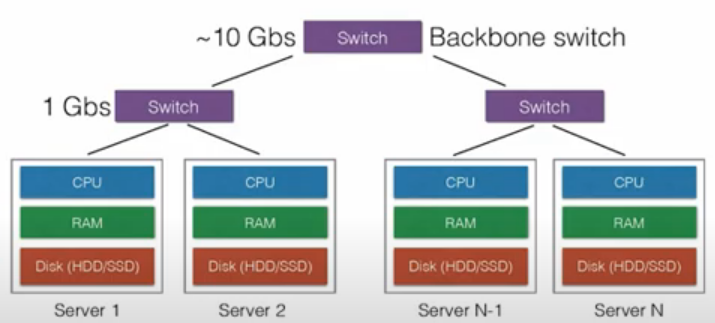
\includegraphics[width=1\textwidth]{parallelisation.png}
\caption{Дата-центр}
\end{figure}

Дата-центр - это множество обычных компьютеров, объединенных rack switch'ом со скоростью передачи 1 Gbs и все это вместе объединено более быстрым switch'ом(Backbone switch) со скоростью 10 Gbs.

\begin{itemize}
    \item Пусть компьютер ломается раз в 3 года
    \item В нашем дата-центре будет 10 000 компьютеров
    \item В итоге каждый день 10 машин будут ломаться
\end{itemize}

В связи с этим возникают 2 проблемы:

\begin{itemize}
    \item Как сохранить данные на сломанном компьютере
    \item Что делать, если один из серверов, на котором что-то считалось 2 дня упал
\end{itemize}

\section{Распределенная файловая система/Distributed file system/DFS}

\subsection{Как хранить данные?}

- Давайте не будем хранить файл на одном сервере. Можно разбить его на 100 частей и если что-то произойдет с одной из машин, то 99\% нашего файла останется - это хорошо.


- Надо делать бэкапы.

\subsection{Самые известные реализации}

\begin{itemize}
    \item GFS(Google file system), придуман гуглом для гугла
    \item HDFS(Hadoop distributed file system), open-source, часть проекта Hadoop
\end{itemize}

Давайте поговорим об HDFS

\subsection{Как работает HDFS}

Давайте загрузим наш файл в HDFS. Далее файл разбивается на чанки размером 64 MB(редко больше или меньше). Потом каждый чанк отправляется на N серверов(в основном на 3). Если один из серверов выйдет из строя, то чанк, который лежал на сервере, отправится на другой сервер, где его еще нет. До отправки чанка на другой сервер у нас все еще будет доступно 2 других машины с данным чанком.
А почему мы отправляем один и тот же чанк на 3 разных сервера? почему не на 2? Шанс того, что два сервера выйдут из строя одновременно выше, чем три.\\

Какие минусы у этой системы? 1 MB теперь будет весить 3 MB. А на самом деле еще больше из-за NameNode.\\

NameNode - сервер, на котором хранится информация о том, где какой чанк хранится

\subsection{Что может пойти не так?}

\begin{enumerate}
    \item BackBone switch(NameNode) отключилась из-за отсутствия питания
    \item BackBone switch(NameNode) проблемы с HDD
    \item Упал Rack Switch - недоступна часть серверов
    \item Проблемы с HDD на машине
\end{enumerate}
1)Ничего страшного, кластер недоступен, но как только появится питание все будет хорошо\\
2)Все плохо, у нас забитые данными серверами, но мы не знаем где какой чанк лежит, можно удалять все и записывать данные заново\\
3)Не критично, у нас есть реплики файлов на других серверах\\
4)Все хорошо, ставим новый HDD, в это время досоздаются утерянные чанки\\

\textit{Исходя из 3 пункта можно понять, что отправлять все чанки одного файла на машины, которые объединены одним rack switch'ом плохая идея, если он(rack switch) упадет, то весь файл будет недоступен.}

\subsection{NameNode x3}

На самом деле NameNode не одна. Всего серверов, которые мы можем назвать NameNode - 3. Работает один сервер, а остальные просто копируют его действия. В случае потери одной NameNode у нас еще будет 2, которые могут ее заменить. А для жесткого диска NameNode делается бэкап.

\begin{figure}[h]
\centering
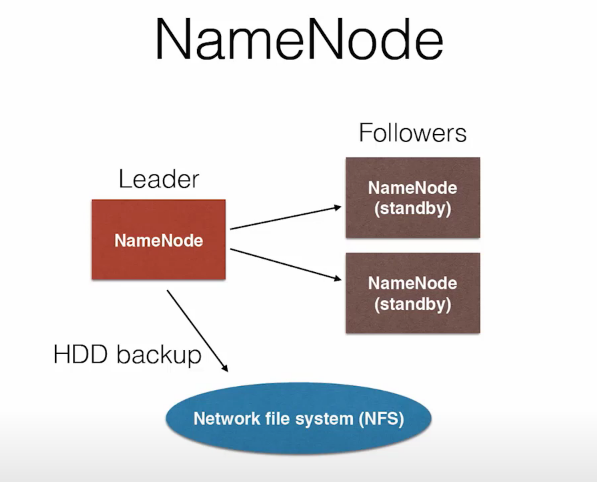
\includegraphics[width=1\textwidth]{NameNode.png}
\caption{NameNodes}
\end{figure}

\section{Расчеты}

\subsection{Параллельная сортировка массивов}

Merge Sort очень хорошо можно распределить на много машин.\\

Результаты Google в сортировке:

\begin{itemize}
    \item 2007: 1 PB / 12.13 часа
    \item 2008: 1 PB / 6.03 часа
    \item 2010: 1 PB / 2.95 часа
    \item 2011: 1 PB / 0.55 часа
    \item 2012: 50 PB / 23 часа
\end{itemize}
А больше сортировать уже не было смысла, весь интернет весил меньше (10 PB), чем они отсортировали в последний раз.

\subsection{MapReduce}

MapReduce - вычислительная модель, которая позволяет решать задачи параллельно и при этом она легко программируема. Была запатентована Google'ом. Про нее \textbf{точно спросят на собеседовании}.\\

Как ни странно, MapReduce состоит из 2 шагов - Map и Reduce.\\

Как работает Map?\\

Допустим, у нас есть входной файл с кучей строк. В каждый момент времени мы обрабатываем только 1 строку и в памяти у нас находится тоже только одна строка. К строке применяется функция Map, которая возвращает пару (ключ, значение).

Далее(где-то между Map и Reduce), полученные пары сортируются по ключам, т.е. сначала идут все записи с ключом 1, ключом 2, ключом 3 и т.д.

После этого для каждого такого "блока" с одинаковыми ключами запускается функция Reduce. Каждый Reduce принимает один такой блок и на выходе мы получаем уникальные пары (ключ, значение) (На примерах все станет понятно).

\begin{figure}[h]
\centering
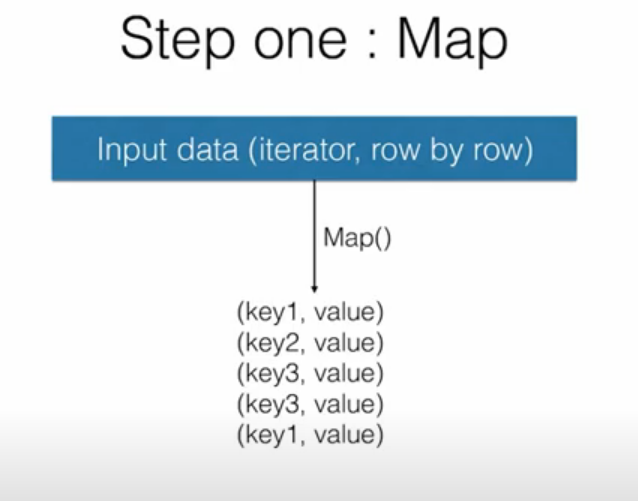
\includegraphics[width=1\textwidth, trim={0 1cm 0 0}, clip]{Map.png}
\caption{Step 1 - Map}

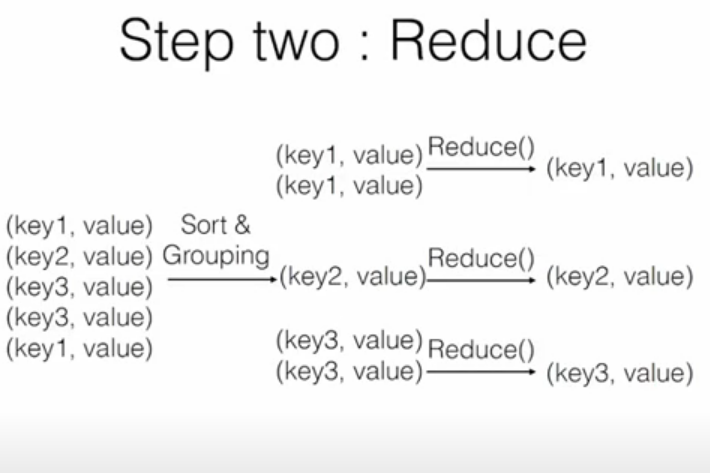
\includegraphics[width=1\textwidth, trim={0 2cm 0 0}, clip]{Reduce.png}
\caption{Step 2 - Reduce}
\end{figure}

\clearpage


\subsection{Примеры}

Допустим, у нас есть международный магазин и данные о магазине, категории проданного товара, количестве проданного товара, цене товара и выручке. И мы хотим посчитать выручку магазинов в каждом городе.

\begin{figure}[h]
\centering
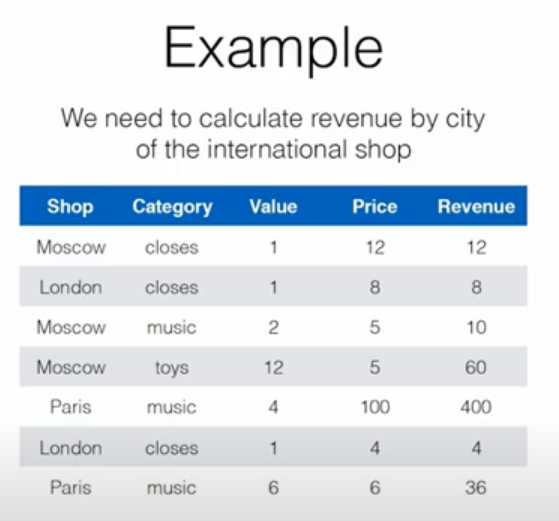
\includegraphics[width=0.85\textwidth, trim={0 0 0 5cm}, clip]{MapReduce_example.png}
\caption{Пример}
\end{figure}

Давайте вытащим из таблички данные о магазине и выручке. Пройдемся маппером, отсортируем полученные пары по ключам и запустим Reduce, который будет суммировать все значения для каждого ключа. В итоге получим выручку магазинов.

\begin{figure}[h]
\centering
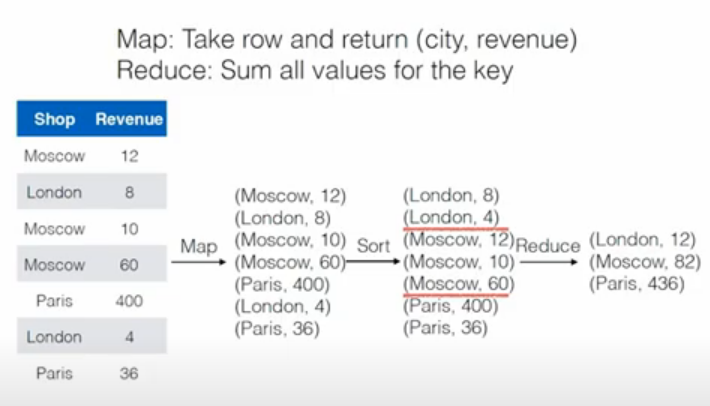
\includegraphics[width=0.85\textwidth]{MapReduce_example2.png}
\caption{Пример}
\end{figure}

На самом деле мы не совсем сортируем пары по ключу и MapReduce работает быстрее, чем MapSortReduce. Мы делаем немного иначе. Давайте возьмем первые 3 записи из таблицы для наглядности(Moscow 12, London 8, Moscow 10). Как только мы встречаем новое значение ключа, например Moscow, мы создаем новый Reducer и отправляем значение(Revenue в нашем случае) в него. После Moscow мы встретим London и снова создадим еще один Reducer. Далее, опять будет Moscow, а мы уже создавали Reducer для такого ключа, поэтому отправляем его туда.\\

Еще примеры:
\begin{enumerate}
    \item Выручка по категории
    \item Выручка в разрезе по магазину, по категории
    \item Средняя выручка по магазину
    \item Найти уникальные магазины(сколько магазинов всего есть)
    \item Гистограмма продаж(сколько магазинов продали от 0 до 100, от 100 до 500 и т.д.)
\end{enumerate}



\noindent Как сделать?\\
1)То же самое, что и в первом примере, но вытаскиваем из таблицы магазин и категорию.\\
2)Составной ключ. Map должен выводить \texttt{Moscow\_toys}, \texttt{Paris\_toys}.\\
3)Проходимся по магазину и по выручке, один Reduce считает количество чисел, а другой сумму выручки и в ответ выведем сумму, деленную на количество чисел.\\
4)Как только Reducer получил уникальный магазин он выдает этот магазин и выключается.\\
5)Проходимся по таблице, видим Moscow 12, значит значение в ключе 0-100 будет равным 1, Paris 400, значение в ключе 100-500 равно 1 и т.д. . И все это отправляется в Reducer, и получается гистограмма.

\subsection{WordCount}

Подсчет количества встречаемых слов в интернете это то, что мы пытались сделать в самом начале. Это своеобразный Hello World в мире MapReduce. На самом деле это довольно понятная задача, Map будет выводить (слово, 1), (другое слово, 1) и т.д., а потом все слова отправить в Reducer, который по сути будет просто суммой. И если у нас есть те самые 10 000 машин, то 1200 дней превращаются в 4 часа.

Однако есть одна проблема, существуют стоп-слова(артикли, союзы, предлоги), которые встречаются очень часто. В википедии есть слово, которое встречается 1e+08 раз, скорее всего это артикль "a" в английском языке, после него идут "the", "to", "for" и другие. Это бессмысленные слова. Мы можем посчитать 99.9\% слов и еще 4 дня мы будем ждать пока посчитается количество артиклей "a". Такие тяжелые случаи называются монстрами и Reducer будет на них страдать. Что делать в таких случаях? Для таких случаев у нас есть Combiners.

Давайте заранее сложим результаты операции Map с одинаковыми ключами, тогда на Reducer у нас придет не больше пар, чем запущено операций Map, и будем все это делать на машине, на которой запущен Map.

\begin{figure}[h]
\centering
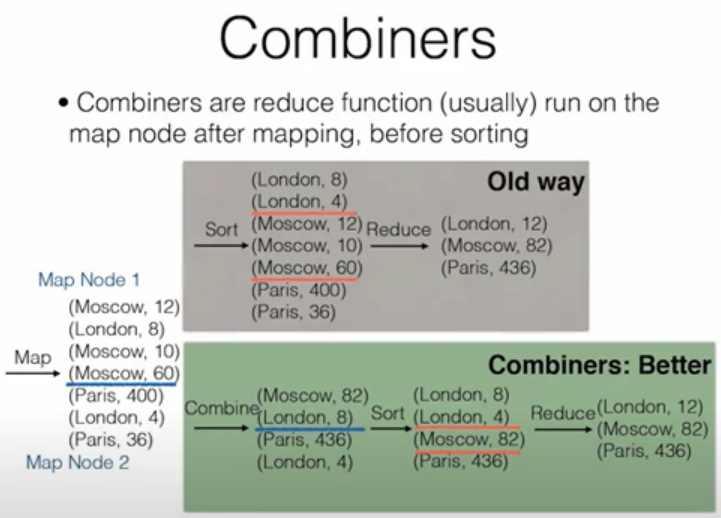
\includegraphics[width=1\textwidth]{Combiners.png}
\caption{Combiner}
\end{figure}

Однако, не все можно сделать с помощью Combiner. Им подчиняются только коммутативные(f(a,b) = f(b,a)) и ассоциативные(f(a,f(b,c))= f(f(a,b),c)) правила. Сумму и произведение легко запустить на MapReduce + Combine, среднее сложнее, например у нас есть следующие значения 3, 3, 3, 1 среднее здесь 2.5, а если запустить на Combiners и в один у нас придет 3, 3, 3, а в другой 1, то он посчитает, что среднее равно 2.
Исправить это можно следующим образом: пусть Combiner считает среднее и количество значений, а затем считает средневзвешенное, т.е. в том примере у нас будет (3 * 3 + 1 * 1)/(3 + 1) = 2.5. Медиану и квантили посчитать нельзя потому что нам одновременно нужны все данные. Однако, можно взять какую-то часть наших данных и на ней посчитать медиану. В больших данных сотая часть это тоже большие данные.

\subsection{Что нам нужно делать?}

Нам ничего не нужно делать, Hadoop все сделает за нас

\begin{itemize}
    \item Разбиение файла на чанки
    \item Какая функция на каком сервере будет запускаться(минимизация трафика в сети)
    \item Группировка и отправка в Reducer
    \item Отлов ошибок
\end{itemize}

\noindent От программиста на Hadoop требуется только написать 2 функции: Map - принимает на вход итератор по строкам, Reduce принимает на вход словарь. Практически на любом языке можно их написать(python, c++, java, bash и  т.д.).

\noindent А что может сломаться внутри машины?
\begin{itemize}
    \item Map Node 
    \item Reduce Node
    \item Master Node(Node, которая следит какие ключи куда отправляются)
\end{itemize}

\noindent Что делать?\\
1)Запускаем на тех же данных, на другой машине с этими данными.\\
2)Аналогично.\\
3)Перезапускаем операцию.

\section{Еще немного про Big Data}

В 80-х годах хранение 1 GB стоило около 100 000\$, а сейчас порядка 0.01 \$. Именно по этой причине мы можем собирать все данные и логи.

\begin{figure}[h]
\centering
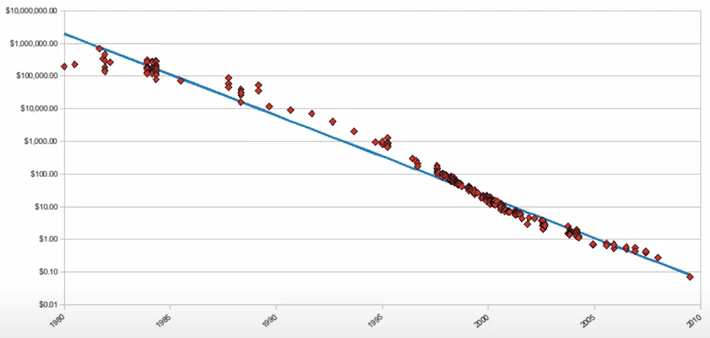
\includegraphics[width=1\textwidth]{why.png}
\caption{Стоимость памяти}
\end{figure}

\subsection{3 самые главные проблемы в Big Data}

\begin{enumerate}
    \item Объем
    \item Разнообразие данных
    \item Скорость
\end{enumerate}

\noindent 1)Цитата лектора - "Много, сложно, параллельно, очень тяжело"\\
2)Вместо названий у вас будут звездочки(*), куча NaN, не экранированные кавычки, огромный JSON файл, в котором одно значение не будет в кавычках. В общем большое количество самых разных проблем в качестве данных. С другой стороны, данных же много, т.е. то, что нам не нравится мы можем просто выкинуть, потеряем 5 \% данных ну и пусть.\\
3)Иногда, данные можно обрабатывать медленно, а иногда нужно сделать это быстро.

\subsection{Корреляции}
В Big Data корреляция даже в 3\% может сказать о том, что переменные действительно связанны.\\

\noindent Забавная история 1.\\

Ребята в Wallmart посмотрели на свои данные и поняли, что продажи пива скоррелированны с продажами подгузников. Не совсем было понятно почему, но нас это мало интересует, раз есть корреляция значит можно на этом заработать. Поставить товары рядом, сделать акцию на покупку пива + подгузников (но люди могут что-то заподозрить).\\

\noindent Забавная история 2.\\

Рекомендательная система Wallmart по покупкам определяет кто вы, что вам нравится, что вам предложить. И они как-то отправили 15-летней девочке поздравление с беременностью и предложили ей соответствующие товары. Отец девочки подал на них в суд и выиграл иск потому что это было вмешательство в личную жизнь. Оказалось, что девочка действительно была беременна. Wallmart узнал об этом раньше родителей.




\end{document}

